\pagebreak
Block name: wta\_new

Number of inputs: 3

Number of outputs: 1

Parameter list: number of blocks, wta\_new\_buf\_bias, wta\_new\_wta\_bias

Block description: 
A vectorized version of WTA circuit. Classic work on winner take all circuit $(https://papers.nips.cc/paper/151-winner-take-all-networks-of-on-complexity.pdf)$ please read it before attempting to compile. 
This WTA has a FG pFET load (wta\_new\_wta\_bias) at the output. Its output is voltage and input is current (usually used with VMM12x1\_wowta).
The output is buffered using ota in a follower configuration (wta\_new\_buf\_bias). The first input and the output are vectorized where as the second and third input are common.



\begin{figure}[H]  % jpg, png, or pdf
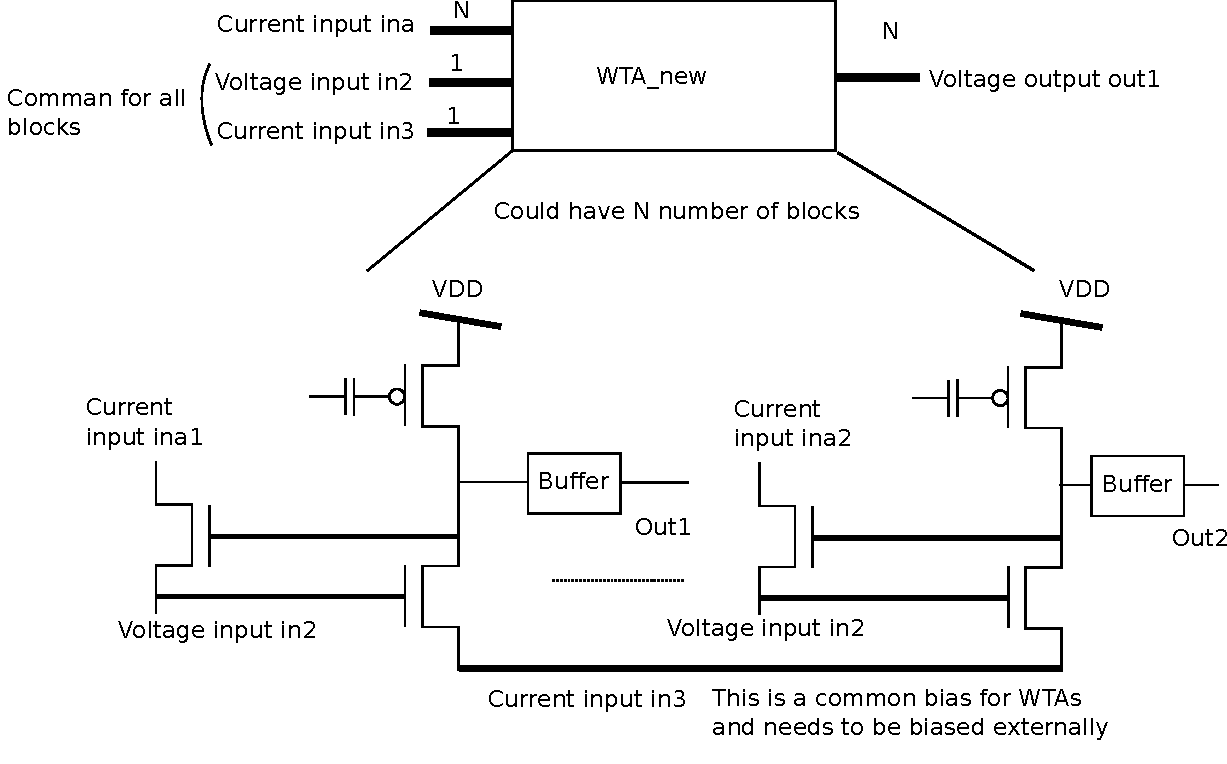
\includegraphics[width=300pt]{$FPAAHOME/rasp30/sci2blif/documentation/blocks_latex/figures/wta_new.pdf}
\end{figure}

